% Created by tikzDevice version 0.12.3.1 on 2022-07-29 15:13:39
% !TEX encoding = UTF-8 Unicode
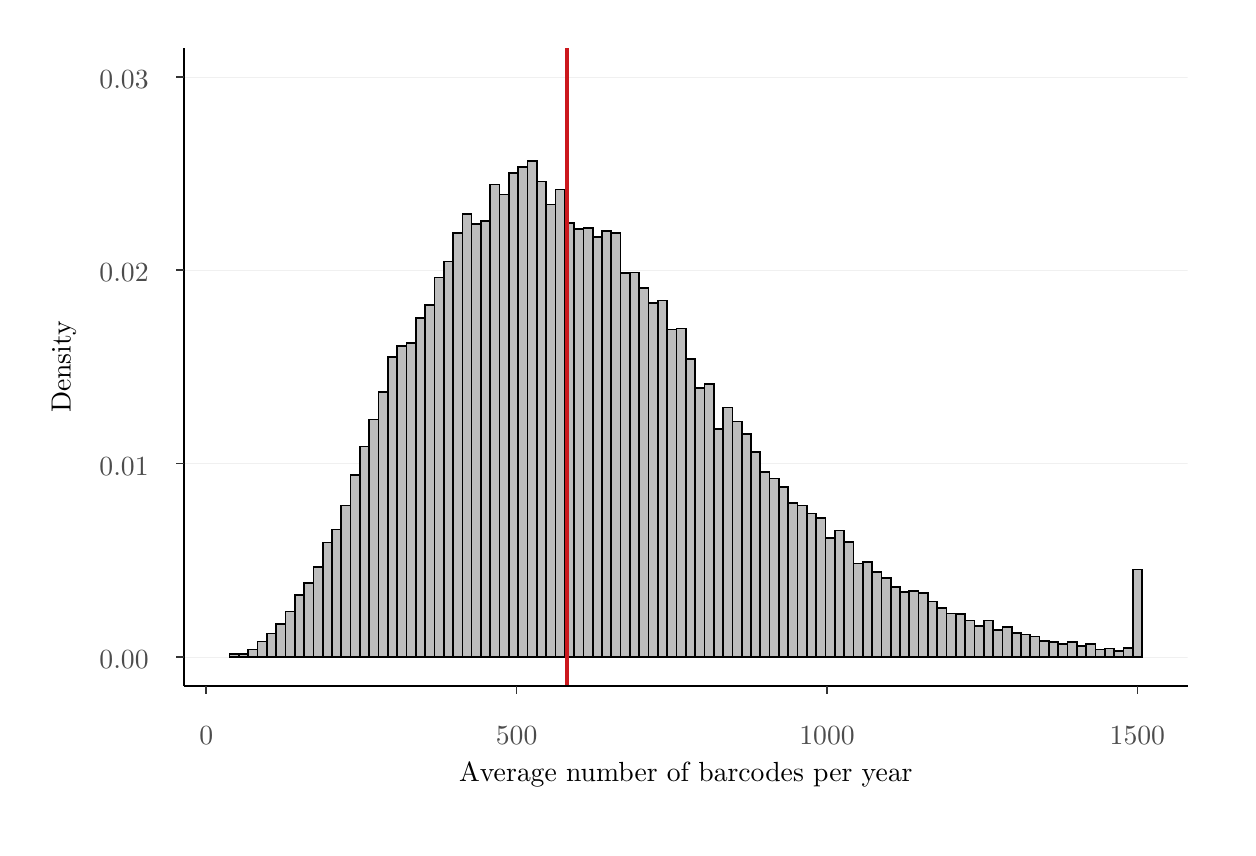
\begin{tikzpicture}[x=1pt,y=1pt]
\definecolor{fillColor}{RGB}{255,255,255}
\path[use as bounding box,fill=fillColor,fill opacity=0.00] (0,0) rectangle (433.62,289.08);
\begin{scope}
\path[clip] (  0.00,  0.00) rectangle (433.62,289.08);
\definecolor{drawColor}{RGB}{255,255,255}
\definecolor{fillColor}{RGB}{255,255,255}

\path[draw=drawColor,line width= 0.6pt,line join=round,line cap=round,fill=fillColor] ( -0.00,  0.00) rectangle (433.62,289.08);
\end{scope}
\begin{scope}
\path[clip] ( 56.47, 51.15) rectangle (419.17,281.85);
\definecolor{drawColor}{RGB}{255,255,255}

\path[draw=drawColor,line width= 0.3pt,line join=round] ( 56.47, 96.59) --
	(419.17, 96.59);

\path[draw=drawColor,line width= 0.3pt,line join=round] ( 56.47,166.50) --
	(419.17,166.50);

\path[draw=drawColor,line width= 0.3pt,line join=round] ( 56.47,236.41) --
	(419.17,236.41);

\path[draw=drawColor,line width= 0.3pt,line join=round] (120.62, 51.15) --
	(120.62,281.85);

\path[draw=drawColor,line width= 0.3pt,line join=round] (232.77, 51.15) --
	(232.77,281.85);

\path[draw=drawColor,line width= 0.3pt,line join=round] (344.92, 51.15) --
	(344.92,281.85);
\definecolor{drawColor}{gray}{0.94}

\path[draw=drawColor,line width= 0.1pt,line join=round] ( 56.47, 61.64) --
	(419.17, 61.64);

\path[draw=drawColor,line width= 0.1pt,line join=round] ( 56.47,131.55) --
	(419.17,131.55);

\path[draw=drawColor,line width= 0.1pt,line join=round] ( 56.47,201.46) --
	(419.17,201.46);

\path[draw=drawColor,line width= 0.1pt,line join=round] ( 56.47,271.37) --
	(419.17,271.37);
\definecolor{drawColor}{RGB}{0,0,0}
\definecolor{fillColor}{gray}{0.74}

\path[draw=drawColor,line width= 0.6pt,line cap=rect,fill=fillColor] ( 72.95, 61.64) rectangle ( 76.32, 62.74);

\path[draw=drawColor,line width= 0.6pt,line cap=rect,fill=fillColor] ( 76.32, 61.64) rectangle ( 79.68, 62.64);

\path[draw=drawColor,line width= 0.6pt,line cap=rect,fill=fillColor] ( 79.68, 61.64) rectangle ( 83.05, 64.33);

\path[draw=drawColor,line width= 0.6pt,line cap=rect,fill=fillColor] ( 83.05, 61.64) rectangle ( 86.41, 67.32);

\path[draw=drawColor,line width= 0.6pt,line cap=rect,fill=fillColor] ( 86.41, 61.64) rectangle ( 89.77, 70.11);

\path[draw=drawColor,line width= 0.6pt,line cap=rect,fill=fillColor] ( 89.77, 61.64) rectangle ( 93.14, 73.60);

\path[draw=drawColor,line width= 0.6pt,line cap=rect,fill=fillColor] ( 93.14, 61.64) rectangle ( 96.50, 78.08);

\path[draw=drawColor,line width= 0.6pt,line cap=rect,fill=fillColor] ( 96.50, 61.64) rectangle ( 99.87, 84.06);

\path[draw=drawColor,line width= 0.6pt,line cap=rect,fill=fillColor] ( 99.87, 61.64) rectangle (103.23, 88.45);

\path[draw=drawColor,line width= 0.6pt,line cap=rect,fill=fillColor] (103.23, 61.64) rectangle (106.60, 94.23);

\path[draw=drawColor,line width= 0.6pt,line cap=rect,fill=fillColor] (106.60, 61.64) rectangle (109.96,103.00);

\path[draw=drawColor,line width= 0.6pt,line cap=rect,fill=fillColor] (109.96, 61.64) rectangle (113.33,107.78);

\path[draw=drawColor,line width= 0.6pt,line cap=rect,fill=fillColor] (113.33, 61.64) rectangle (116.69,116.45);

\path[draw=drawColor,line width= 0.6pt,line cap=rect,fill=fillColor] (116.69, 61.64) rectangle (120.06,127.41);

\path[draw=drawColor,line width= 0.6pt,line cap=rect,fill=fillColor] (120.06, 61.64) rectangle (123.42,137.78);

\path[draw=drawColor,line width= 0.6pt,line cap=rect,fill=fillColor] (123.42, 61.64) rectangle (126.79,147.54);

\path[draw=drawColor,line width= 0.6pt,line cap=rect,fill=fillColor] (126.79, 61.64) rectangle (130.15,157.31);

\path[draw=drawColor,line width= 0.6pt,line cap=rect,fill=fillColor] (130.15, 61.64) rectangle (133.51,169.96);

\path[draw=drawColor,line width= 0.6pt,line cap=rect,fill=fillColor] (133.51, 61.64) rectangle (136.88,174.05);

\path[draw=drawColor,line width= 0.6pt,line cap=rect,fill=fillColor] (136.88, 61.64) rectangle (140.24,175.05);

\path[draw=drawColor,line width= 0.6pt,line cap=rect,fill=fillColor] (140.24, 61.64) rectangle (143.61,184.22);

\path[draw=drawColor,line width= 0.6pt,line cap=rect,fill=fillColor] (143.61, 61.64) rectangle (146.97,188.80);

\path[draw=drawColor,line width= 0.6pt,line cap=rect,fill=fillColor] (146.97, 61.64) rectangle (150.34,198.86);

\path[draw=drawColor,line width= 0.6pt,line cap=rect,fill=fillColor] (150.34, 61.64) rectangle (153.70,204.55);

\path[draw=drawColor,line width= 0.6pt,line cap=rect,fill=fillColor] (153.70, 61.64) rectangle (157.07,214.81);

\path[draw=drawColor,line width= 0.6pt,line cap=rect,fill=fillColor] (157.07, 61.64) rectangle (160.43,221.69);

\path[draw=drawColor,line width= 0.6pt,line cap=rect,fill=fillColor] (160.43, 61.64) rectangle (163.80,218.10);

\path[draw=drawColor,line width= 0.6pt,line cap=rect,fill=fillColor] (163.80, 61.64) rectangle (167.16,219.19);

\path[draw=drawColor,line width= 0.6pt,line cap=rect,fill=fillColor] (167.16, 61.64) rectangle (170.52,232.35);

\path[draw=drawColor,line width= 0.6pt,line cap=rect,fill=fillColor] (170.52, 61.64) rectangle (173.89,228.76);

\path[draw=drawColor,line width= 0.6pt,line cap=rect,fill=fillColor] (173.89, 61.64) rectangle (177.25,236.63);

\path[draw=drawColor,line width= 0.6pt,line cap=rect,fill=fillColor] (177.25, 61.64) rectangle (180.62,238.63);

\path[draw=drawColor,line width= 0.6pt,line cap=rect,fill=fillColor] (180.62, 61.64) rectangle (183.98,240.82);

\path[draw=drawColor,line width= 0.6pt,line cap=rect,fill=fillColor] (183.98, 61.64) rectangle (187.35,233.54);

\path[draw=drawColor,line width= 0.6pt,line cap=rect,fill=fillColor] (187.35, 61.64) rectangle (190.71,225.17);

\path[draw=drawColor,line width= 0.6pt,line cap=rect,fill=fillColor] (190.71, 61.64) rectangle (194.08,230.55);

\path[draw=drawColor,line width= 0.6pt,line cap=rect,fill=fillColor] (194.08, 61.64) rectangle (197.44,218.60);

\path[draw=drawColor,line width= 0.6pt,line cap=rect,fill=fillColor] (197.44, 61.64) rectangle (200.81,216.40);

\path[draw=drawColor,line width= 0.6pt,line cap=rect,fill=fillColor] (200.81, 61.64) rectangle (204.17,216.60);

\path[draw=drawColor,line width= 0.6pt,line cap=rect,fill=fillColor] (204.17, 61.64) rectangle (207.53,213.51);

\path[draw=drawColor,line width= 0.6pt,line cap=rect,fill=fillColor] (207.53, 61.64) rectangle (210.90,215.71);

\path[draw=drawColor,line width= 0.6pt,line cap=rect,fill=fillColor] (210.90, 61.64) rectangle (214.26,214.81);

\path[draw=drawColor,line width= 0.6pt,line cap=rect,fill=fillColor] (214.26, 61.64) rectangle (217.63,200.46);

\path[draw=drawColor,line width= 0.6pt,line cap=rect,fill=fillColor] (217.63, 61.64) rectangle (220.99,200.56);

\path[draw=drawColor,line width= 0.6pt,line cap=rect,fill=fillColor] (220.99, 61.64) rectangle (224.36,194.98);

\path[draw=drawColor,line width= 0.6pt,line cap=rect,fill=fillColor] (224.36, 61.64) rectangle (227.72,189.70);

\path[draw=drawColor,line width= 0.6pt,line cap=rect,fill=fillColor] (227.72, 61.64) rectangle (231.09,190.49);

\path[draw=drawColor,line width= 0.6pt,line cap=rect,fill=fillColor] (231.09, 61.64) rectangle (234.45,180.03);

\path[draw=drawColor,line width= 0.6pt,line cap=rect,fill=fillColor] (234.45, 61.64) rectangle (237.82,180.43);

\path[draw=drawColor,line width= 0.6pt,line cap=rect,fill=fillColor] (237.82, 61.64) rectangle (241.18,169.27);

\path[draw=drawColor,line width= 0.6pt,line cap=rect,fill=fillColor] (241.18, 61.64) rectangle (244.55,158.90);

\path[draw=drawColor,line width= 0.6pt,line cap=rect,fill=fillColor] (244.55, 61.64) rectangle (247.91,160.20);

\path[draw=drawColor,line width= 0.6pt,line cap=rect,fill=fillColor] (247.91, 61.64) rectangle (251.27,143.95);

\path[draw=drawColor,line width= 0.6pt,line cap=rect,fill=fillColor] (251.27, 61.64) rectangle (254.64,151.83);

\path[draw=drawColor,line width= 0.6pt,line cap=rect,fill=fillColor] (254.64, 61.64) rectangle (258.00,146.75);

\path[draw=drawColor,line width= 0.6pt,line cap=rect,fill=fillColor] (258.00, 61.64) rectangle (261.37,142.26);

\path[draw=drawColor,line width= 0.6pt,line cap=rect,fill=fillColor] (261.37, 61.64) rectangle (264.73,135.78);

\path[draw=drawColor,line width= 0.6pt,line cap=rect,fill=fillColor] (264.73, 61.64) rectangle (268.10,128.51);

\path[draw=drawColor,line width= 0.6pt,line cap=rect,fill=fillColor] (268.10, 61.64) rectangle (271.46,126.22);

\path[draw=drawColor,line width= 0.6pt,line cap=rect,fill=fillColor] (271.46, 61.64) rectangle (274.83,123.13);

\path[draw=drawColor,line width= 0.6pt,line cap=rect,fill=fillColor] (274.83, 61.64) rectangle (278.19,117.25);

\path[draw=drawColor,line width= 0.6pt,line cap=rect,fill=fillColor] (278.19, 61.64) rectangle (281.56,116.45);

\path[draw=drawColor,line width= 0.6pt,line cap=rect,fill=fillColor] (281.56, 61.64) rectangle (284.92,113.56);

\path[draw=drawColor,line width= 0.6pt,line cap=rect,fill=fillColor] (284.92, 61.64) rectangle (288.28,111.87);

\path[draw=drawColor,line width= 0.6pt,line cap=rect,fill=fillColor] (288.28, 61.64) rectangle (291.65,104.69);

\path[draw=drawColor,line width= 0.6pt,line cap=rect,fill=fillColor] (291.65, 61.64) rectangle (295.01,107.38);

\path[draw=drawColor,line width= 0.6pt,line cap=rect,fill=fillColor] (295.01, 61.64) rectangle (298.38,103.30);

\path[draw=drawColor,line width= 0.6pt,line cap=rect,fill=fillColor] (298.38, 61.64) rectangle (301.74, 95.42);

\path[draw=drawColor,line width= 0.6pt,line cap=rect,fill=fillColor] (301.74, 61.64) rectangle (305.11, 96.02);

\path[draw=drawColor,line width= 0.6pt,line cap=rect,fill=fillColor] (305.11, 61.64) rectangle (308.47, 92.43);

\path[draw=drawColor,line width= 0.6pt,line cap=rect,fill=fillColor] (308.47, 61.64) rectangle (311.84, 90.24);

\path[draw=drawColor,line width= 0.6pt,line cap=rect,fill=fillColor] (311.84, 61.64) rectangle (315.20, 87.05);

\path[draw=drawColor,line width= 0.6pt,line cap=rect,fill=fillColor] (315.20, 61.64) rectangle (318.57, 85.26);

\path[draw=drawColor,line width= 0.6pt,line cap=rect,fill=fillColor] (318.57, 61.64) rectangle (321.93, 85.56);

\path[draw=drawColor,line width= 0.6pt,line cap=rect,fill=fillColor] (321.93, 61.64) rectangle (325.29, 84.86);

\path[draw=drawColor,line width= 0.6pt,line cap=rect,fill=fillColor] (325.29, 61.64) rectangle (328.66, 81.67);

\path[draw=drawColor,line width= 0.6pt,line cap=rect,fill=fillColor] (328.66, 61.64) rectangle (332.02, 79.28);

\path[draw=drawColor,line width= 0.6pt,line cap=rect,fill=fillColor] (332.02, 61.64) rectangle (335.39, 77.39);

\path[draw=drawColor,line width= 0.6pt,line cap=rect,fill=fillColor] (335.39, 61.64) rectangle (338.75, 77.29);

\path[draw=drawColor,line width= 0.6pt,line cap=rect,fill=fillColor] (338.75, 61.64) rectangle (342.12, 74.89);

\path[draw=drawColor,line width= 0.6pt,line cap=rect,fill=fillColor] (342.12, 61.64) rectangle (345.48, 72.80);

\path[draw=drawColor,line width= 0.6pt,line cap=rect,fill=fillColor] (345.48, 61.64) rectangle (348.85, 74.89);

\path[draw=drawColor,line width= 0.6pt,line cap=rect,fill=fillColor] (348.85, 61.64) rectangle (352.21, 71.41);

\path[draw=drawColor,line width= 0.6pt,line cap=rect,fill=fillColor] (352.21, 61.64) rectangle (355.58, 72.60);

\path[draw=drawColor,line width= 0.6pt,line cap=rect,fill=fillColor] (355.58, 61.64) rectangle (358.94, 70.41);

\path[draw=drawColor,line width= 0.6pt,line cap=rect,fill=fillColor] (358.94, 61.64) rectangle (362.30, 69.81);

\path[draw=drawColor,line width= 0.6pt,line cap=rect,fill=fillColor] (362.30, 61.64) rectangle (365.67, 69.11);

\path[draw=drawColor,line width= 0.6pt,line cap=rect,fill=fillColor] (365.67, 61.64) rectangle (369.03, 67.42);

\path[draw=drawColor,line width= 0.6pt,line cap=rect,fill=fillColor] (369.03, 61.64) rectangle (372.40, 67.02);

\path[draw=drawColor,line width= 0.6pt,line cap=rect,fill=fillColor] (372.40, 61.64) rectangle (375.76, 66.42);

\path[draw=drawColor,line width= 0.6pt,line cap=rect,fill=fillColor] (375.76, 61.64) rectangle (379.13, 67.02);

\path[draw=drawColor,line width= 0.6pt,line cap=rect,fill=fillColor] (379.13, 61.64) rectangle (382.49, 65.73);

\path[draw=drawColor,line width= 0.6pt,line cap=rect,fill=fillColor] (382.49, 61.64) rectangle (385.86, 66.32);

\path[draw=drawColor,line width= 0.6pt,line cap=rect,fill=fillColor] (385.86, 61.64) rectangle (389.22, 64.43);

\path[draw=drawColor,line width= 0.6pt,line cap=rect,fill=fillColor] (389.22, 61.64) rectangle (392.59, 64.73);

\path[draw=drawColor,line width= 0.6pt,line cap=rect,fill=fillColor] (392.59, 61.64) rectangle (395.95, 63.83);

\path[draw=drawColor,line width= 0.6pt,line cap=rect,fill=fillColor] (395.95, 61.64) rectangle (399.32, 64.83);

\path[draw=drawColor,line width= 0.6pt,line cap=rect,fill=fillColor] (399.32, 61.64) rectangle (402.68, 93.33);
\definecolor{drawColor}{RGB}{203,24,29}

\path[draw=drawColor,line width= 1.7pt,line join=round] (194.86, 51.15) -- (194.86,281.85);
\end{scope}
\begin{scope}
\path[clip] (  0.00,  0.00) rectangle (433.62,289.08);
\definecolor{drawColor}{RGB}{0,0,0}

\path[draw=drawColor,line width= 0.6pt,line join=round] ( 56.47, 51.15) --
	( 56.47,281.85);
\end{scope}
\begin{scope}
\path[clip] (  0.00,  0.00) rectangle (433.62,289.08);
\definecolor{drawColor}{gray}{0.30}

\node[text=drawColor,anchor=base east,inner sep=0pt, outer sep=0pt, scale=  1.00] at ( 43.72, 57.51) {0.00};

\node[text=drawColor,anchor=base east,inner sep=0pt, outer sep=0pt, scale=  1.00] at ( 43.72,127.42) {0.01};

\node[text=drawColor,anchor=base east,inner sep=0pt, outer sep=0pt, scale=  1.00] at ( 43.72,197.32) {0.02};

\node[text=drawColor,anchor=base east,inner sep=0pt, outer sep=0pt, scale=  1.00] at ( 43.72,267.23) {0.03};
\end{scope}
\begin{scope}
\path[clip] (  0.00,  0.00) rectangle (433.62,289.08);
\definecolor{drawColor}{gray}{0.20}

\path[draw=drawColor,line width= 0.6pt,line join=round] ( 53.72, 61.64) --
	( 56.47, 61.64);

\path[draw=drawColor,line width= 0.6pt,line join=round] ( 53.72,131.55) --
	( 56.47,131.55);

\path[draw=drawColor,line width= 0.6pt,line join=round] ( 53.72,201.46) --
	( 56.47,201.46);

\path[draw=drawColor,line width= 0.6pt,line join=round] ( 53.72,271.37) --
	( 56.47,271.37);
\end{scope}
\begin{scope}
\path[clip] (  0.00,  0.00) rectangle (433.62,289.08);
\definecolor{drawColor}{RGB}{0,0,0}

\path[draw=drawColor,line width= 0.6pt,line join=round] ( 56.47, 51.15) --
	(419.17, 51.15);
\end{scope}
\begin{scope}
\path[clip] (  0.00,  0.00) rectangle (433.62,289.08);
\definecolor{drawColor}{gray}{0.20}

\path[draw=drawColor,line width= 0.6pt,line join=round] ( 64.54, 48.40) --
	( 64.54, 51.15);

\path[draw=drawColor,line width= 0.6pt,line join=round] (176.69, 48.40) --
	(176.69, 51.15);

\path[draw=drawColor,line width= 0.6pt,line join=round] (288.85, 48.40) --
	(288.85, 51.15);

\path[draw=drawColor,line width= 0.6pt,line join=round] (401.00, 48.40) --
	(401.00, 51.15);
\end{scope}
\begin{scope}
\path[clip] (  0.00,  0.00) rectangle (433.62,289.08);
\definecolor{drawColor}{gray}{0.30}

\node[text=drawColor,anchor=base,inner sep=0pt, outer sep=0pt, scale=  1.00] at ( 64.54, 30.14) {0};

\node[text=drawColor,anchor=base,inner sep=0pt, outer sep=0pt, scale=  1.00] at (176.69, 30.14) {500};

\node[text=drawColor,anchor=base,inner sep=0pt, outer sep=0pt, scale=  1.00] at (288.85, 30.14) {1000};

\node[text=drawColor,anchor=base,inner sep=0pt, outer sep=0pt, scale=  1.00] at (401.00, 30.14) {1500};
\end{scope}
\begin{scope}
\path[clip] (  0.00,  0.00) rectangle (433.62,289.08);
\definecolor{drawColor}{RGB}{0,0,0}

\node[text=drawColor,anchor=base,inner sep=0pt, outer sep=0pt, scale=  1.00] at (237.82, 16.79) {Average number of barcodes per year};
\end{scope}
\begin{scope}
\path[clip] (  0.00,  0.00) rectangle (433.62,289.08);
\definecolor{drawColor}{RGB}{0,0,0}

\node[text=drawColor,rotate= 90.00,anchor=base,inner sep=0pt, outer sep=0pt, scale=  1.00] at ( 15.49,166.50) {Density};
\end{scope}
\end{tikzpicture}
